\chapter*{Wstęp}

Medycyna w Polsce jest dobrze rozwinięta, ale nie zawsze osoby, potrzebujące pomocy, otrzymują tę pomoc w najszybszym czasie. W rankingu tak zwanego zrównoważonego rozwoju systemów ochrony zdrowia Polska zajmuje 25 miejsce na 28 państw UE. Wychodząc z tego, pomysł projektu polega na zwracaniu dodatkowej uwagi tematu zdrowia, który został na takim poziomie w 2020 roku, na którym był w 2012.

\begin{figure}[!ht]
	\centering
		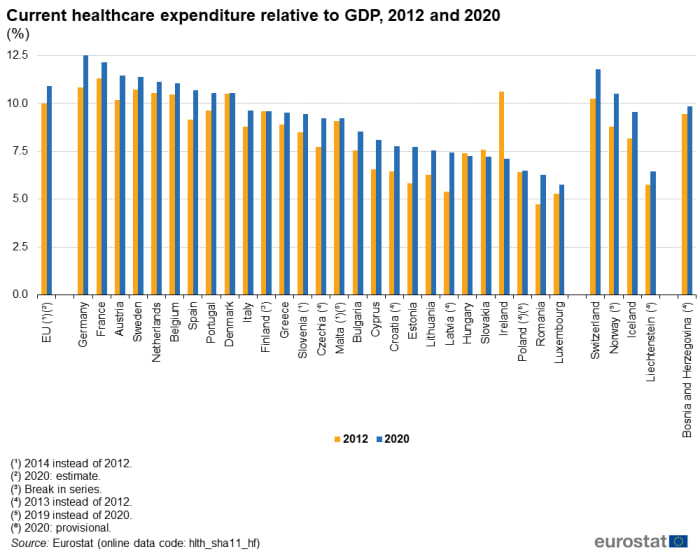
\includegraphics[width=16cm]{polska_med.jpg}
	\caption{\footnotesize Porównanie poziomu ochrony zdrowia pomiędzy krajami UE. Żródło: \cite{www-1}}
	\label{fig:plotend}
\end{figure}

Ignorowanie rozwoju tematów, powiązanych ze zdrowiem, może spowodować stracone życia, które udałoby uratować, gorsze wydarzenie o Polsce, jako o kraju w całości, powolnienie wykonywania prac we wszystkich obszarach biznesu i nie tylko.
